\section{77 - MAT - AG 2.5, AN 1.1, AN 1.3, FA 1.4, FA 1.5, FA 1.7, FA 3.2 - Kettenlinie - BIFIE Aufgabensammlung}

\begin{langesbeispiel} \item[0] %PUNKTE DES BEISPIELS
	
Hängt man ein Seil (oder beispielsweise eine Kette) an zwei Punkten auf, so kann der Verlauf des Seils unter bestimmten Bedingungen durch eine Funktion der Form $x\mapsto \frac{a}{2}\cdot\left(e^\frac{x}{a}+e^-\frac{x}{a}\right)$ mit $a\in\mathbb{R}^+$ modelliert werden.

Der Wert der Konstanten $a$ hängt dabei von der Seillänge und vom Abstand der beiden Aufhängepunkte ab.

Der vertikale Abstand zwischen dem tiefsten Punkt des Seils und seinen Aufhängepunkten wird als Durchhang bezeichnet.

Ein bestimmtes Seil kann modellhaft durch eine Funktion $f$ der obigen Form mit $a=4$ beschrieben werden ($x$ und $f(x)$ in Metern). Die beiden Aufhängepunkte $P_1$ und $P_2$ befinden sich in gleicher Höhe und ihr Abstand beträgt $d=6$\,cm.

\subsection{Aufgabenstellung:}
\begin{enumerate}
	\item Gib eine Gleichung an, mit der die Stelle mit dem maximalen Durchhang des durch $f$ beschriebenen Seils berechnet werden kann, und ermittle diese Stelle!\leer
	
	Gib eine Funktionsgleichung $f_1$ an, mit der ein Seil modelliert werden kann, welches an jeweils 1\,m tieferen Aufhängepunkten montiert ist und denselben Durchhang wie das durch $f$ beschriebene Seil aufweist!\leer
	
	\item Gib eine Gleichung an, mit der der Durchhang $\delta_1$, der die Abhängigkeit des Durchhangs von der Länge des Seils zwischen den Aufhängepunkten $P_1$ und $P_2$ beschreibt.
	
\begin{center}
	\resizebox{0.9\linewidth}{!}{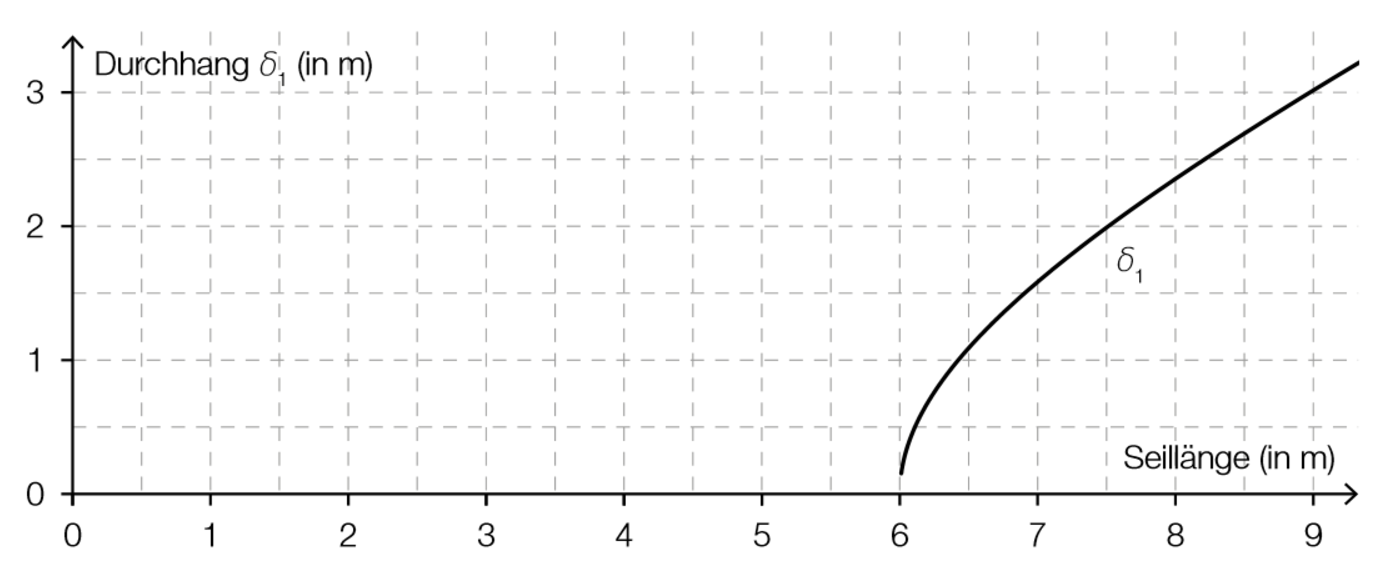
\includegraphics{../Bilder/Bild77-1.eps}}
\end{center}
	
	Gib mithilfe der oben dargestellten Abbildung die Länge des in der Einleitung beschriebenen Seils an! Ermittle weiters, um wie viele Meter der Durchhang zunimmt, wenn das Seil durch ein zwei Meter längeres Seil (gleicher Beschaffenheit) ersetzt wird, das an denselben Aufhängepunkten montiert ist!\leer
	
	\item Der Graph der Funktion $f$ kann durch den Graphen einer quadratischen Funktion $g$ mit $g(x)=b\cdot x²+c$ mit $b,c\in\mathbb{R}^+$ angenähert werden. Der Graph von $g$ verläuft durch die Aufhängepunkte $P_1$ und $P_2$ und den Tiefpunkt des Graphen von $f$.\leer
	
	Gib alle Gleichungen an, die für die Berechnung von $b$ und $c$ notwendig sind, und ermittle die Werte dieser Parameter!\leer
	
	Gib eine Gleichung an, mit der der größte vertikale Abstand von $f$ und $g$ zwischen den beiden Aufhängepunkten berechnet werden kann!\leer
	
	\item Der Graph der Funktion $f$ kann auch durch den Graphen einer Polynomfunktion $f$ vierten Grades angenähert werden. Für den Graphen von $h$ gelten folgende Bedingungen: er verläuft durch die Aufhängepunkte $P_1$ und $P_2$ und den Tiefpunkt des Graphen von $f$ und hat in den beiden Aufhängepunkten dieselbe Steigung wie der Graph von $f$.\leer
	
	Drücke \underline{alle} gegebenen Bedingungen mithilfe von Gleichungen aus!\leer
	
	Ermittle anhand dieser Gleichungen eine Funktionsgleichung von $h$!
	
\end{enumerate}

\antwort{
\begin{enumerate}
	\item \subsection{Lösungserwartung:} 

$f'(x)=\frac{1}{2}\cdot\left(e^{\frac{x}{4}}+e^{-\frac{x}{4}}\right)=0 \Rightarrow x=0$

$f_1(x)=f(x)-1=\frac{4}{2}\cdot\left(e^{\frac{x}{4}}+e^{-\frac{x}{4}}\right)-1$

	\item \subsection{Lösungserwartung:}
	
	$\delta=f(3)-f(0)$
	
	$\delta=1,2$\,m\leer
	
	Die Seillänge beträgt ca. 6,6\,m.
	
	$\delta_1(8,6)\approx 2,8 \Rightarrow$ Der Durchhang nimmt um ca. 1,6\,m zu.

\item \subsection{Lösungserwartung:}
	
$g(0)=4=c$\leer

$g(3)=f(3)\approx 5,18=9\cdot b+4 \Rightarrow b\approx 0,13$\leer

größter vertikaler Abstand:

$(g(x)-f(x))'=0$

\item \subsection{Lösungserwartung:}
	
$h(-3)=f(-3)$

$h(0)=f(0)$

$h(3)=f(3)$

$h'(-3)=f'(-3)$

$h'(3)=f'(3)$\leer

$h(x)\approx 0,0007\cdot x^4+0,125\cdot x²+4$

\end{enumerate}}
		\end{langesbeispiel}